\section{Introduction}
\label{sec:intro}
Electromigration (EM) is a physical phenomenon that the metal atoms migrate along the direction of several driving forces, such as the applied electrical field. 
With the complexity of modern very large scale integration (VLSI) designs, EM remains the top reliability failure mechanism for copper-based interconnects in all the sub-nanometer technologies.
As a consequence of the EM effect, when the hydrostatic stress inside the metal wire reaches the critical level, resistance may varies over time during the migration, and the conducting electrons at the cathode and anode will form a void and a hillock.
The EM crisis becomes even worse as technology advances to smaller manufacturing processes. 
%The International Roadmap for Devices and Systems (IRDS) \cite{IRDS20} predicts that the allowable current density will continue to decrease due to EM, while the required current density to drive the gates will continue to increase. Developing and employing more accurate EM models and less conservative EM sign-off and assessment techniques for EM-aware designs and runtime management is critical. 

On chip power distribution networks (PDN) is a mesh-structured network, which provide power to transistors from top metals, are usually vulnerable to the EM-induced failures, since the current on the PDN are large and unidirectional. In order to design robust PDN, designers have to properly size the PDN wires to meet the area and IR drop requirement. This task is changeling as the wires resistance may change along the time due to the EM effect, resulting in IR drops go blow the threshold after years of aging effect. 

\begin{figure}[htp]
	\centering
	\subfigure[]{
		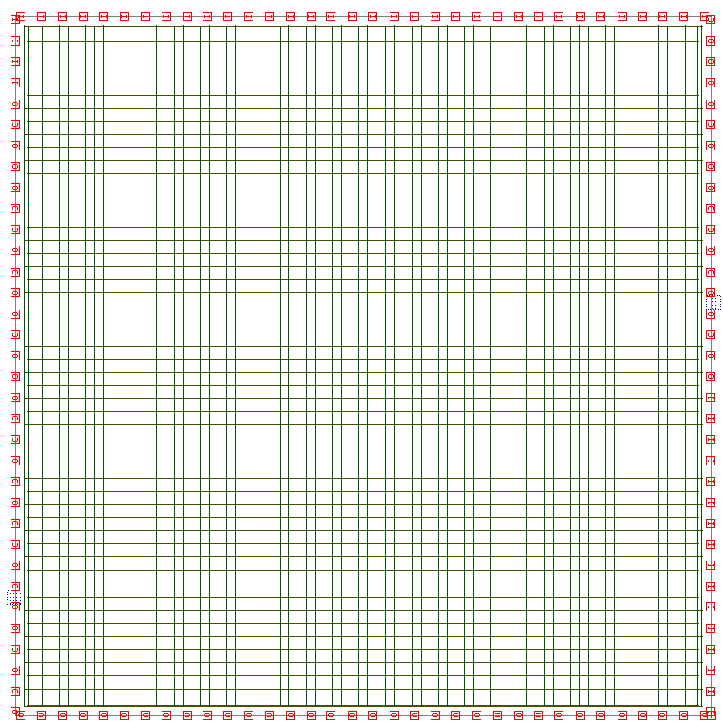
\includegraphics[width=0.4\columnwidth]{./figs/icc2pg.eps}
		\label{fig:icc2pg}}
	\subfigure[]{
		\includegraphics[width=0.48\columnwidth]{./figs/genpg.eps}
		\label{fig:genpg}}
	\caption{(a) Power and ground networks of Cortex-M0 DesignStart; (b) Voltage drop map of the power network of (a).}
	\label{fig:pgimage}
\end{figure}


Many past research works tried to address the EM-aware PDN reliability issue based analytical methods, such as nonlinear or sequence of linear programming (SLP) methods~\cite{ChBr:TCAD'88,DuMa:DAC'89,Tan:DAC'99,Wang:TCAD'05,ZhouSun:TVLSI'19, Sukharev:2019pg, ZhouYu:ASPDAC'20,ZhouJin:ICCAD'20}. Zhou {\it et al.}~\cite{ZhouSun:TVLSI'19,ZhouChen:Integration'21} proposed a power grid network sizing method based on a multi-segment EM immortality check criteria. Moudallal {\it et al.}~\cite{Sukharev:2019pg} proposed to directly consider EM-induced IR drops instead of EM constraints on the time-varying power grid networks. It can consider post-voiding resistance change of wires based on finite difference analysis of EM-induced stress in multi-segment wires, and the resulting nonlinear problem is solved by applying successive linear programming. This method, however, may suffer high computational costs as the sensitivities of those violating nodes need to be computed by solving the circuit matrices. This computation workload of matrices construction and matrices solving increases polynomially as the size of the power grid increases. 
   
Recently, Zhou {\it et al.} proposed a localized machine learning-accelerated EM-aware IR drop fixing method for power grid networks. The optimization is carried out based on the sensitivities method in which the sensitivities were computed by the generative adversarial network (GAN)-based model called {\it GridNet}. This method was initially only applied to localized optimization, and it has been extended to full-chip optimization~\cite{HanLiu:TCAD'22-23}.  The method shows the promise of leveraging machine learning acceleration in the field of power grid optimization.

However they are some drawbacks of GAN-based strategy, such as GANs are challenging to train due to the need to optimize opposing objectives of the generator and discriminator, leading to issues like mode collapse. Recently,  (VAE) gained much traction as it has the training and better interpretability of latent space, compare to the contemporaries, such as GAN, which provides them with a robust mathematical grounding and better generated result in some scenarios. 

Based on those observations, we propose a fast EM-aware full-chip power grid IR drop fixing method by leveraging the modeling power of VAE. Our key contributions are decomposed as follows:

\begin{itemlist}
	


%We propose using a conditional generative adversarial network(CGAN)-based tool {\it GridNet}~\cite{ZhouJin:ICCAD'20} to quickly acquire the sensitivity matrix for the power grid fixing, avoiding a heavy-loaded numerical computation process and improving the running speed.

%\item First we propose a VAE-based model to fast predict the EM-aware full-chip power grid IR drop. Our new model reduced approximately 40$\%$ RMSE in mV, Compared to the GAN-based model.
\item We propose a VAE-based IR-drop modeling framework which can fast predict the on chip power grid IR-drop considering EM effect, achieve over 40$\%$ reduction in RMSE over state-of-the-art GAN-based model.   
	
%\item Second, instead of using the circuit matrix solving-based sensitivity computation method in~\cite{Sukharev:2019pg}, we quickly acquired the sensitivity information from the network auto-gradient,  which is similar to the CGAN in ~\cite{ZhouJin:ICCAD'20}, to compute the EM-induced IR drop at the given lifetime and the sensitivities of the IR drops with respect to the wire segment width.  Our VAE-based strategy significantly improves the running speed of the current SLP-based voltage failure fixing methods.
\item We accelerated the SLP method for full-chip power grid IR drop failure fixing by fast acquiring the sensitivity matrix from the VAE model back propagation. 
 Experimental results on a number of synthesized power grid benchmarks from ARM Cortex-M0 processor designs show that the proposed method can provide up to 90X (at least one order of magnitude) speedup over the existing analytical matrix solving-based SLP method ~\cite{Sukharev:2019pg}.
 And it scales well  with a large number of violations and thereby improving the efficiency of the whole optimization process.
    %Compared to the recently proposed GAN-accelerated conjugate gradient-based optimization method, the proposed method can lead to 2-8X speedup on the synthesized power grid networks.
  
\end{itemlist}

The rest of the paper is organized as follows:
Section~\ref{sec:related} reviews the related preliminary works on the
EM-induced IR drop analysis and current EM-aware power grid
optimization strategy. Section~\ref{sec:strategy} introduces the
VAE-based EM-aware IR drop prediction method. Experiment setup, numerical results, as long as
analysis and discussions are summarized in Section~\ref{sec:results}.
Section~\ref{sec:conclusion} concludes the paper.
